\section{Detalji penjačkog smjera}

\begin{figure}[H]
    \centering
    \includegraphics[width=0.3\textwidth]{images/implementacija/route-details/route-details.png}
    \caption{Detalji penjačkog smjera na mobilnoj aplikaciji}
    \label{fig:detalji_smjera}
\end{figure}

Pristupom detaljnom pregledu pojedinog penjačkog smjera na mobilnoj aplikaciji (slika~\ref{fig:detalji_smjera}), korisniku se prikazuju informacije o penjačkom smjeru. Na vrhu zaslona istaknuti su osnovni podaci poput naziva, lokacije u obliku imena penjačke lokacije i sektora, težine te tip penjačkog smjera. 
U pozadini se nalazi referentna slika penjačkog smjera. Klikom na pozadinu nestaju sve informacije o penjačkom smjeru kako bi slika postala vidljiva. Ispod toga, aplikacija nudi detaljni uvid u karakteristike penjačkog smjera koristeći oznake za opisivanje stila penjanja. Neke od karakteristika su veliki hvatovi, tehnički potezi, mali hvatovi i kosa stijena. Karakteristike određuju penjači koji su upisali da su popeli penjački smjer.

\begin{figure}[H]
    \centering
    \includegraphics[width=0.8\textwidth]{images/implementacija/web/route-details/route-details.png}
    \caption{Detalji penjačkog smjera na web aplikaciji}
    \label{fig:detalji_smjera_web}
\end{figure}

Na web aplikaciji korisniku se prikazuju iste informacije, no one se nalaze u listi penjačkih smjerova kada je označen pregled određenog sektora na stranici detalja penjačke lokacije (slika~\ref{fig:detalji_smjera_web}). Klikom na penjački smjer u listi, korisniku se na lijevo prikazuje referentna slika penjačkog smjera.

\begin{figure}[H]
    \centering
    \begin{subfigure}[b]{0.38\textwidth}
        \centering
        \includegraphics[width=\textwidth]{images/implementacija/route-details/log-ascent.png}
        \caption{Mobilna aplikacija}
        \label{fig:formular_uspona_mob}
    \end{subfigure}
    \hfill
    \begin{subfigure}[b]{0.55\textwidth}
        \centering
        \includegraphics[width=\textwidth]{images/implementacija/web/route-details/log-ascent.png}
        \caption{Web aplikacija}
        \label{fig:formular_uspona_web}
    \end{subfigure}
    \caption{Formular za unos podataka o usponu}
    \label{fig:formular_uspona}
\end{figure}

Klikom na gumb "Zapiši uspon" (eng. \textit{Log Ascent}) ili na web aplikaciji izbornik u kartici penjačkog smjera, korisnik pristupa formi za unos podataka o usponu (slika~\ref{fig:formular_uspona}). Za unos uspona potrebno je odabrati datum i stil uspona. Opcije za stil uspona su \textit{Flash}, \textit{Onsight}, \textit{Redpoint} i \textit{Aid}. Korisnik također može unijeti broj pokušaja koje je imao na penjačkom smjeru, dati ocjenu u obliku broja zvjezdica te odabrati karakteristike penjačkog smjera. Finalno korisnik može unijeti neki komentar uspona što može uključivati neka upozorenja ili pohvale za kvalitetu penjačkog smjera.

\begin{figure}[H]
    \centering
    \begin{subfigure}[b]{0.38\textwidth}
        \centering
        \includegraphics[width=\textwidth]{images/implementacija/route-details/view-ascents.png}
        \caption{Mobilna aplikacija}
        \label{fig:prikaz_uspona_mob}
    \end{subfigure}
    \hfill
    \begin{subfigure}[b]{0.55\textwidth}
        \centering
        \includegraphics[width=\textwidth]{images/implementacija/web/route-details/view-ascents.png}
        \caption{Web aplikacija}
        \label{fig:prikaz_uspona_web}
    \end{subfigure}
    \caption{Prikaz uspona}
    \label{fig:prikaz_uspona}
\end{figure}

Klikom na gumb za prikaz uspona u gornjem desnom kutu zaslona ili klikom na gumb za prikaz uspona u kartici penjačkog smjera na web aplikaciji, korisniku se prikazuje popis uspona na tom penjačkom smjeru (slika~\ref{fig:prikaz_uspona}). Popis sadrži zabilježene uspon svih korisnika na tom penjačkom smjeru sortirano po datumu uspona od najnovije prema najstarijem. Svaki unos sadrži korisničko ime, stil uspona, predloženu težinu, karakteristike penjačkog smjera koje je korisnik unio, osobni komentar i broj zvjezdica.
